\documentclass[11pt, twoside, pdftex]{article}

% This include all the settings that we should use for the document
\newcommand{\PDFTitle}{Using PCI Express on DE4 Boards}
\newcommand{\commonPath}{../../Common}
\newcommand{\datePublished}{Mar 2022}

\newcommand{\versnum}{21.1} %version number quartus/AMP
\newcommand{\quartusname}{Quartus\textsuperscript{\textregistered} Prime}	
\newcommand{\textBar}{For \quartusname{} \versnum{}}
\newcommand{\thisyear}{2022 } %for copyright
\newcommand{\company}{FPGAcademy.org}
\newcommand{\longteamname}{FPGAcademy.org}
\newcommand{\teamname}{FPGAcademy}
\newcommand{\website}{FPGAcademy.org}

\newcommand{\productAcronym}{AMP}
\newcommand{\productNameShort}{Monitor Program}

\newcommand{\productNameMedTM}{Monitor Program}
\newcommand{\productNameMed}{Monitor Program}

%\newcommand{\headerLogoFilePath}[1]{#1/FPGAcademy.png}



\setlength\topmargin{-0.25in}
\setlength\headheight{0in}
\setlength\headsep{0.35in}
\setlength\textheight{8.5in}
\setlength\textwidth{7in}
\setlength\oddsidemargin{-0.25in}
\setlength\evensidemargin{-0.25in}
\setlength\parindent{0.25in}
\setlength\parskip{0in} 

\pdfpagewidth 8.5in
\pdfpageheight 11in

% listings is a package that supports encapsulating source code in LaTeX conveniently

\usepackage{listings}
% add support for graphics
\usepackage{graphicx}
\usepackage[usenames, dvipsnames]{color}

\def\expandparam\lstinputlisting[#1]#2{\edef\tmp{\noexpand\lstinputlisting[#1]{#2}}\tmp}

\widowpenalty 10000
\clubpenalty 10000

%%%%%%%%%%%%%%%%%%%% Source Code Formatting %%%%%%%%%%%%%%%%%%%%
\definecolor{globalCommentColour}{rgb}{0.588,0.588,0.588}

%%%%%%%%%%%%%%%%%%%%%%%%%%%%%%%%%%%%%%%%%%%%%%%%%%%%
% Defining a NiosII ASM highlighter for lstlisting
\lstdefinelanguage[NiosII]{Assembler} {
 	morekeywords={add, addi, and, andhi, andi, beq, bge, bgeu, bgt, bgtu, ble,  bleu, blt, bltu, bne, br, break,% 
 	bret, call, callr, cmpeq, cmpeqi, cmpge, cmpgei, cmpgeu, cmpgeui, cmpgt, cmpgti, cmpgtu, cmpgtui, cmple,%
 	cmplei, cmpleu, cmpleui, cmplt, cmplti, cmpltu, cmpltui, cmpne, cmpnei, custom, div, divu, eret, flushd,%
 	flushda, flushi, flushp, initd, initda, initi, jmp, jmpi, ldb, ldbio, ldbu, ldbuio, ldh, ldhio, ldhu, ldhuio,%
 	ldw, ldwio, mov, movhi, movi, movia, movui, mul, muli, mulxss, mulxsu, mulxuu, nextpc, nop, nor, or, orhi, ori,%
 	rdctl, rdprs, ret, rol, roli, ror, sll, slli, sra, srai, srl, srli, stb, stbio, sth, sthio, stw, stwio,%
 	sub, subi, sync, trap, wrctl, wrtcl, wrprs, xor, xori, xorhi, xori},% 	
 	morekeywords=[2]{.abort, .ABORT, .align, .app-file, .ascii, .asciz, .balign, .byte, .comm, .data, .def,%
 	.desc, .dim, .double, .eject, .else, .end, .endef, .endif, .equ, .equiv, .err, .extern, .file, .fill, .float,%
 	.global, .globl, .hword, .ident, .if, .include, .int, .irp, .irpc, .lcomm, .lflags, .line, .linkonce, .ln,%
 	.list, .long, .macro, .mri, .nolist, .octa, .org, .p2align, .psize, .quad, .rept, .sbttl, .scl, .section,%
 	.set, .short, .single, .size, .sleb128, .skip, .space, .stadb, .stabn, .stabs, .string, .symver, .tag,%
 	.text, .title, .type, .val, .uleb128, .word},% 	
 	morekeywords=[3]{et, bt, gp, sp, fp, ea, sstatus, ra, pc, status, estatus, bstatus, ienable, ipending, cpuid,%
 	exception, pteaddr, tlbacc, tlbmisc, eccinj, badaddr, config, mpubase, mpuacc},% 	
 	sensitive=t,%
 	alsoletter=.,%
	morestring=[b]",%
 	morecomment=[s]{/*}{*/},%
 	morecomment=[l]\#,%
   }[keywords,comments,strings]
   
   %% NOTE: morekeywords=[2] are GNU directives.
   
   \definecolor{niosInstructionColour}{rgb}{0.000,0.608,0.000}
   \definecolor{niosDirectiveColour}{rgb}{0.000,0.000,0.902}
   \definecolor{niosSpecialRegColour}{rgb}{0.000,0.000,0.000}
   \definecolor{niosStringColour}{rgb}{0.808,0.482,0.000}
   
   %% NOTE: To make bold use: =\bfseries\color{<colour>}
   \lstdefinestyle{defaultNiosStyle} {
   language=[NiosII]{Assembler},
   stringstyle=\color{niosStringColour},
   keywordstyle=\color{niosInstructionColour},
   keywordstyle=[2]\color{niosDirectiveColour},
   keywordstyle=[3]\itshape\color{niosSpecialRegColour}
   }
%%%%%%%%%%%%%%%%%%%%%%%%%%%%%%%%%%%%%%%%%%%%%%%%%%%%

%%%%%%%%%%%%%%%%%%%%%%%%%%%%%%%%%%%%%%%%%%%%%%%%%%%%
% Defining a ArmA9 ASM highlighter for lstlisting
\lstdefinelanguage[ArmA9]{Assembler} {
 	morekeywords={ADC, ADD, ADDS, AND, ANDS, B, BAL, BEQ, BGE, BGT, BL, BLT, BIC, BKPT, BLX, BNE, BX, CDP, CLZ, CMN, CMP, EOR,%
 	EORS, LDC, LDM, LDR, LDRB, LDRBT, LDRH, LDRSB, LDRSH, LDRT, LSL, MCR, MLA, MOV, MOVW, MOVT, MRC, MRS, MSR, MUL, MVN, ORR, PLD,%
 	ROR, RSB, RSC, SBC, SMLAL, SMULL, STC, STM, STR, STRB, STRBT, STRH, STRT, SUB, SUBS, SWI, SWP, SWPB, TEQ, UMLAL,
 	PUSH, POP, MOVS, RORS, LSR},%
 	morekeywords=[2]{.abort, .ABORT, .align, .app-file, .ascii, .asciz, .balign, .byte, .comm, .data, .def,%
 	.desc, .dim, .double, .eject, .else, .end, .endef, .endif, .equ, .equiv, .err, .extern, .file, .fill, .float,%
 	.global, .globl, .hword, .ident, .if, .include, .int, .irp, .irpc, .lcomm, .lflags, .line, .linkonce, .ln,%
 	.list, .long, .macro, .mri, .nolist, .octa, .org, .p2align, .psize, .quad, .rept, .sbttl, .scl, .section,%
 	.set, .short, .single, .size, .sleb128, .skip, .space, .stadb, .stabn, .stabs, .string, .symver, .tag,%
 	.text, .title, .type, .val, .vectors, .uleb128, .word},%
 	morekeywords=[3]{SP, PC, MIDR, CTR, TCMTR, TLBTR, MPIDR, ID_PFR0, ID_PFR1, ID_DFR0, ID_MMFR0, ID_MMFR1, ID_MMFR2,%
 	ID_MMFR3, ID_ISAR0, ID_ISAR1, ID_ISAR2, ID_ISAR3, ID_ISAR4, CCSIDR, CLIDR, AIDR, CSSELR, TTBR0, TTRB1, TTBR2, DACR,%
 	DFSR, IFSR, ADFSR, AIFSR, DFAAR, IFAR, ICIALLUIS, BPIALLIS, PAR, ICIALLU, ICIMVAU, BPIALL, DCIMVAC, DCISW, V2PCWPR,%
 	DCCVAC, DCCSW, DDIMVAC, DCISW, TLBALLIS, TLBIMVAIS, TLBIASIDIS, TLBIMVAAIS, TLBIALL, TLBIMVA, TLBIASID, TLBIMVAA,%
 	PMCR, PMCNTENSET, PMCNTENCLR, PMOVSR, PMSWINC, PMSELR, PMXEVTYPER, PMXEVCNTR, PMUSERENR, PMINTENSET, PMINTENCLR,%
 	PRRR, NRRR, PLEIDR, PLEASR, PLEFSR, PLEUAR, PLEPCR, VBAR, MVBAR, ISR, FCSEIDR, CONTEXTIDR, TPIDRURW, TPIDRURO, TPIDRPRW},%
 	sensitive=f,%
 	alsoletter=.,%
	morestring=[b]",%
 	morecomment=[s]{/*}{*/},%
 	morecomment=[l]{//},%
   }[keywords,comments,strings]
   
   %% NOTE: morekeywords=[2] are GNU directives.
   
   \definecolor{armInstructionColour}{rgb}{0.000,0.608,0.000}
   \definecolor{armDirectiveColour}{rgb}{0.000,0.000,0.902}
   \definecolor{armSpecialRegColour}{rgb}{0.000,0.000,0.000}
   \definecolor{armStringColour}{rgb}{0.808,0.482,0.000}
   
   \lstdefinestyle{defaultArmStyle} {
   language=[ArmA9]{Assembler},
   stringstyle=\color{armStringColour},
   keywordstyle=\color{armInstructionColour},
   keywordstyle=[2]\color{armDirectiveColour},
   keywordstyle=[3]\itshape\color{armSpecialRegColour}
   }
%%%%%%%%%%%%%%%%%%%%%%%%%%%%%%%%%%%%%%%%%%%%%%%%%%%%

%%%%%%%%%%%%%%%%%%%%%%%%%%%%%%%%%%%%%%%%%%%%%%%%%%%%
% Defining style for the verilog.

\definecolor{verilogCommentColour}{rgb}{0.000,0.502,0.000}

\lstdefinestyle{defaultVerilogStyle} {
language={Verilog},
keywordstyle=\color{blue},
commentstyle=\color{verilogCommentColour}
}
%%%%%%%%%%%%%%%%%%%%%%%%%%%%%%%%%%%%%%%%%%%%%%%%%%%%

%%%%%%%%%%%%%%%%%%%%%%%%%%%%%%%%%%%%%%%%%%%%%%%%%%%%
% Defining style for the vhdl.
\lstdefinestyle{defaultVHDLStyle} {
language={VHDL},
keywordstyle=\color{blue},
commentstyle=\color{verilogCommentColour}
}
%%%%%%%%%%%%%%%%%%%%%%%%%%%%%%%%%%%%%%%%%%%%%%%%%%%%

%%%%%%%%%%%%%%%%%%%%%%%%%%%%%%%%%%%%%%%%%%%%%%%%%%%%
% Java
\definecolor{javaStringColour}{rgb}{0.808,0.482,0}
%%%%%%%%%%%%%%%%%%%%%%%%%%%%%%%%%%%%%%%%%%%%%%%%%%%%

%%%%%%%%%%%%%%%%%%%%%%%%%%%%%%%%%%%%%%%%%%%%%%%%%%%%
% Defining language styles
% C
\definecolor{CStringColour}{rgb}{0.808,0.482,0}
%%%%%%%%%%%%%%%%%%%%%%%%%%%%%%%%%%%%%%%%%%%%%%%%%%%%

%%%%%%%%%%%%%%%%%%%%%%%%%%%%%%%%%%%%%%%%%%%%%%%%%%%%
% Defining extended LaTeX language.
\lstdefinelanguage[LocalLaTeX]{TeX}[LaTeX]{TeX}%
 	{moretexcs={bf, it, sf, lstset},%
   	}%

\lstdefinestyle{defaultLocalLatexStyle} {
language=[LocalLatex]{TeX},
keywordstyle=\color{blue}\bfseries,
keywordstyle=[2]\color{blue},
keywordstyle=[3]\color{blue}\bfseries
}
%%%%%%%%%%%%%%%%%%%%%%%%%%%%%%%%%%%%%%%%%%%%%%%%%%%%

\lstset{
%language = C,
%language = Verilog,
%basicstyle=\color{black}\rmfamily\ttfamily,
basicstyle=\small\color{black}\ttfamily,
commentstyle=\small\color{globalCommentColour}\itshape\ttfamily,
keywordstyle=\small\color{blue}\bfseries\ttfamily,
showstringspaces=false,
frame=none, %lines % boxed listings
breaklines=true,
breakatwhitespace=true,
tabsize=4
}
%%%%%%%%%%%%%%%%%%%%%%%%%%%%%%%%%%%%%%%%%%%%%%%%%%%%%%%%%%%%%%%%


%\usepackage[centering]{geometry}.
%%%%%%%%%%%%%%%%%%%%%%%%%%%%%%%%%%%%%%%%%%%%%%%%%%%
% Document Settings
\usepackage[labelsep=period]{caption}
% we can choose a better font later
%\usepackage{palatino}
\usepackage{fourier}
%\fontencoding{T1}
% include common used symbols
\usepackage{textcomp}
% add support for graphics
\usepackage{graphicx}
\usepackage[usenames, dvipsnames]{color}
% enable to draw thick or thin table hlines
\setlength{\doublerulesep}{\arrayrulewidth}
\usepackage{longtable}
\setlongtables
%\usepackage{array}
% It may be better to use PDFLaTeX as it can generate bookmarks for the
% document

% Add some useful packages
\usepackage{ae,aecompl}
\usepackage{epsfig,float,times}

% reset the font for section
\usepackage{sectsty}
%\allsectionsfont{\fontfamily{ptm}\selectfont}
\allsectionsfont{\usefont{OT1}{phv}{bc}{n}\selectfont}

% use compact space for sections
\usepackage[compact]{titlesec}
\titlespacing{\section}{0pt}{0.2in}{*0}
\titlespacing{\subsection}{0pt}{0.1in}{*0}
\titlespacing{\subsubsection}{0pt}{0.05in}{*0}

% fancyhdr header and footer customization
\usepackage{layout}
\usepackage{fancyhdr}
\pagestyle{fancy}
\fancyhead{}
\fancyhead[R]{\textit{\tiny{\textBar}}}
\fancyfoot{}
\fancyfoot[LO,
RE]{\textrm{\href{https://www.fpgacademy.org}{\small \longteamname}} \\ {\small \datePublished }}
\fancyfoot[RO, LE]{\small \thepage}
% two-side settings
%\fancyhead{} % clear all header fields
%\fancyfoot{} % clear all footer fields
%\fancyfoot[LE,RO]{\thepage}
\renewcommand{\headrulewidth}{2pt}
\renewcommand{\headrule}{{\color{blue} \hrule width\headwidth height\headrulewidth \vskip-\headrulewidth}}
\renewcommand{\footrulewidth}{0pt}

% Format the footer on page 1
\fancypagestyle{plain}{
\fancyhead{}
\fancyfoot{}
\fancyfoot[LO,
RE]{\textrm{\href{https://www.fpgacademy.org}{\small \longteamname}} \\ {\small \datePublished }}
\fancyfoot[RO, LE]{\small \thepage}
\renewcommand{\headrulewidth}{0pt}
}
% adjust some setting to try to make the figure stay in the same page with text
% Reference: 	http://www.cs.uu.nl/~piet/floats/node1.html
%   			http://mintaka.sdsu.edu/GF/bibliog/latex/floats.html
%   General parameters, for ALL pages:
\renewcommand{\topfraction}{0.9}	% max fraction of floats at top
\renewcommand{\bottomfraction}{0.8}	% max fraction of floats at bottom
%   Parameters for TEXT pages (not float pages):
\setcounter{topnumber}{3}
\setcounter{bottomnumber}{3}
\setcounter{totalnumber}{5}     % 2 may work better
\setcounter{dbltopnumber}{2}    % for 2-column pages
\renewcommand{\dbltopfraction}{0.9}	% fit big float above 2-col. text
\renewcommand{\textfraction}{0.07}	% allow minimal text w. figs
%   Parameters for FLOAT pages (not text pages):
\renewcommand{\floatpagefraction}{0.7}	% require fuller float pages
% N.B.: floatpagefraction MUST be less than topfraction !!
\renewcommand{\dblfloatpagefraction}{0.7}	% require fuller float pages
%%%%%%%%%%%%%%%%%%%%%%%%%%%%%%%%%%%%%%%%%%%%%%%%%%%
% remember to use [htp] or [htpb] for placement
%%%%%%%%%%%%%%%%%%%%%%%%%%%%%%%%%%%%%%%%%%%%%%%%%%%

% set no indent for paragraph
\setlength{\parindent}{0em}
\addtolength{\parskip}{11pt}
\newcommand{\compact}{[topsep=0pt]}
% use this package to reduce space
\usepackage{enumitem}
\usepackage{multirow}
\usepackage{rotating}
\usepackage{pifont}
\usepackage{dingbat}
\newcommand{\itemsecond}{$\circ$}
%
%%%%%%%%%%%%%%%%%%
\date{}
\author{}
%%%%%%%%%%%%%%%%%%
\newcommand{\de}{DE-series}
\newcommand{\up}{FPGAcademy}
\newcommand{\fabric}{Avalon Switch Fabric}
\newcommand{\TODO}[1]{\textcolor{red}{\textbf{TODO}: #1}}
\def\registered{{\ooalign{\hfil\raise .00ex\hbox{\scriptsize R}\hfil\crcr\mathhexbox20D}}}

% enable url and reference(bookmarks) in pdf
\usepackage{url}
\usepackage[pdftex, colorlinks]{hyperref}
\hypersetup{%
pdftitle={\PDFTitle},
linkcolor=blue,
hyperindex=true,
pdfauthor={\longteamname},
pdfkeywords={FPGAcademy, Academic Program, Example System},
bookmarksnumbered,
bookmarksopen=false,
filecolor=blue,
pdfstartview={FitH},
urlcolor=blue,
plainpages=false,
pdfpagelabels=true,
linkbordercolor={1 1 1} %no color for link border
}%
%%%%%%%%%%%%%%%%%%%%%%%%%%%%%%%%%%%%%%%%%%%%%%%%%%%
\setlength{\fboxsep}{0.7pt}
\setlength{\fboxrule}{0.5pt}

\newcommand{\red}[1]{{\color{red}\sf{#1}}}
\newcommand{\blue}[1]{{\color{blue}\sf{#1}}}



%%%%%%%%%%%%%%%%%%%%%%%%%
% Add title
\newcommand{\doctitle}{Using PCI Express\\on DE4 Boards}
\newcommand{\dochead}{Using PCI Express on DE4 Boards}
% Usually no need to change these two lines
\title{\fontfamily{phv}\selectfont{\doctitle} }
\chead{ \small{\textsc{\bfseries \dochead} } }
% Customizations
%%%%%%%%%%%%%%%%%%%%%%%%%
% Allows multiple figures per page

\renewcommand\floatpagefraction{.9}
\renewcommand\topfraction{.9}
\renewcommand\bottomfraction{.9}
\renewcommand\textfraction{.1}   
\setcounter{totalnumber}{50}
\setcounter{topnumber}{50}
\setcounter{bottomnumber}{50}
\widowpenalty 10000
\clubpenalty 10000
\raggedbottom

%%%%%%%%%%%%%%%%%%
%%% DOCUMENT START
%\begin{document}
\begin{document}
\begin{table}
    \centering
    \begin{tabular}{p{5cm}p{4cm}}
        \hspace{-3cm}
        &
        \raisebox{1\height}{\parbox[h]{0.5\textwidth}{\Large\fontfamily{phv}\selectfont{\textsf{\doctitle}}}}
    \end{tabular}
    \label{tab:logo}
\end{table}

\colorbox[rgb]{0,0.384,0.816}{\parbox[h]{\textwidth}{\color{white}\textsf{\textit{\textBar}}}}

\thispagestyle{plain}
 
\section{Introduction}
This tutorial describes how to use the PCI Express (Peripheral Component Interconnect) on Intel DE4 board. It first demonstrates how to build a system with the PCI Express IP Core using Platform Designer and then shows how to use the PCI driver on Linux* operating system. The discussion is based on the assumption that the reader has the basic knowledge of C language and Verilog hardware description language. Also the reader should be familiar with Quartus\textsuperscript{\textregistered} Prime software and Linux operating system.

\noindent
{\bf Contents}:

\begin{itemize}
	\item Background
	\item Building the PCI Express System
	\item Using the Driver
	\item Changing the Driver Codes
\end{itemize}
\clearpage

\section{Background}
PCI Express is a high-performance interconnect protocol for use in a variety of applications including network adapters, storage area networks, embedded controllers, graphic accelerator boards, and audio-video products. 

An example of a system using PCI Express on DE4 board is shown in Figure~\ref{fig:system_block_diagram}. The PCI Express IP Core implements the PCI Express interface protocol to allows data transfer between a host computer and the on-chip memory on the board. The data can be transferred either directly or through the DMA controllers. Besides, a Nios\textsuperscript{\textregistered} II processor is used to perform calculation on the data in the on-chip memory. 

\begin{figure}[H]
	\centering
	  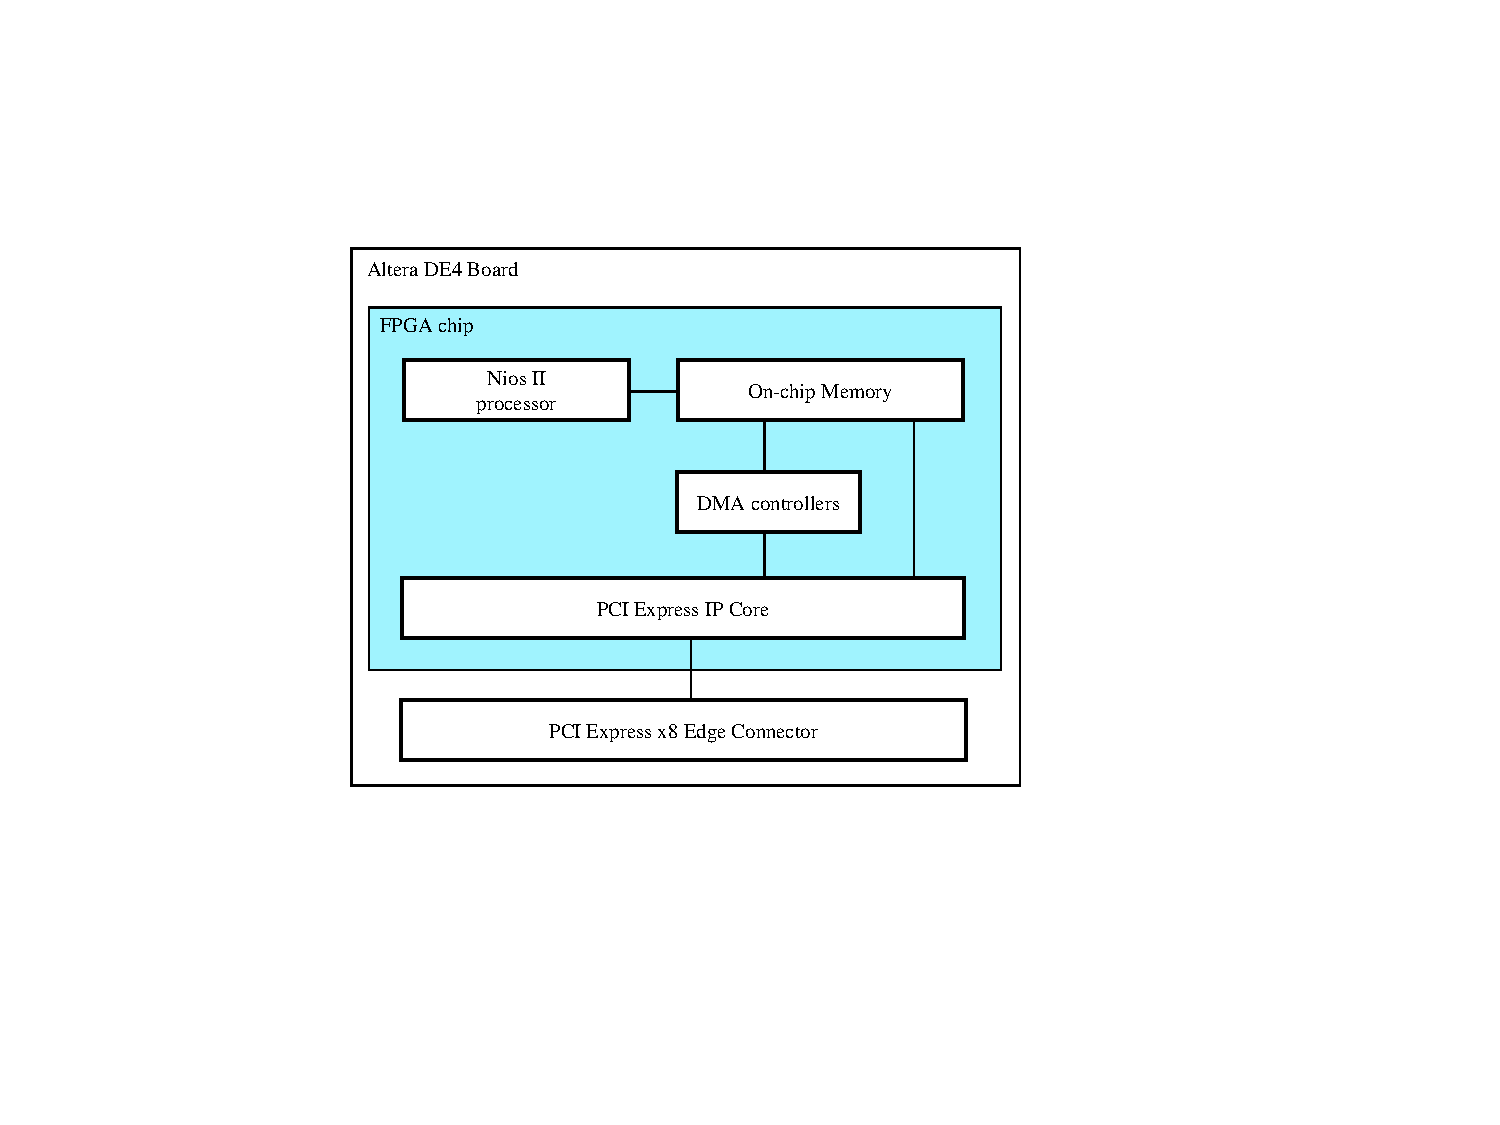
\includegraphics[scale=1]{figures/system_block_diagram.pdf}
	\caption{The block diagram for the system.} 
	\label{fig:system_block_diagram}
\end{figure}

A simple application of this system is that the host computer can put data to the on-chip memory through a DMA controller and wait for the Nios II processor to perform calculation on the data. Once the data is calculated, the host computer can read the data back through the PCI Express IP Core.

Note that this tutorial shows the ways to use both DMA Controller and Scatter-Gather DMA Controller. In a real design, two different kinds of DMA controllers are not necessary. 

\newpage
\section{Building the PCI Express System}
To use the PCI Express on the DE4 board, you have to instantiate the PCI Express IP Core in your hardware system. To start with, create a new Quartus Prime project for your system. As shown in Figure~\ref{fig:create_project}, store your project in a directory called {\it de4\_pcie\_tutorial} and assign the same name to both the project and its top-level design entity. In your project, from the list of available devices, choose the appropriate device name for the FPGA used on the DE4 board. A list of devices names of DE4 boards can be found in Table~\ref{tab:device}.

\begin{figure}[H]
	\centering
	  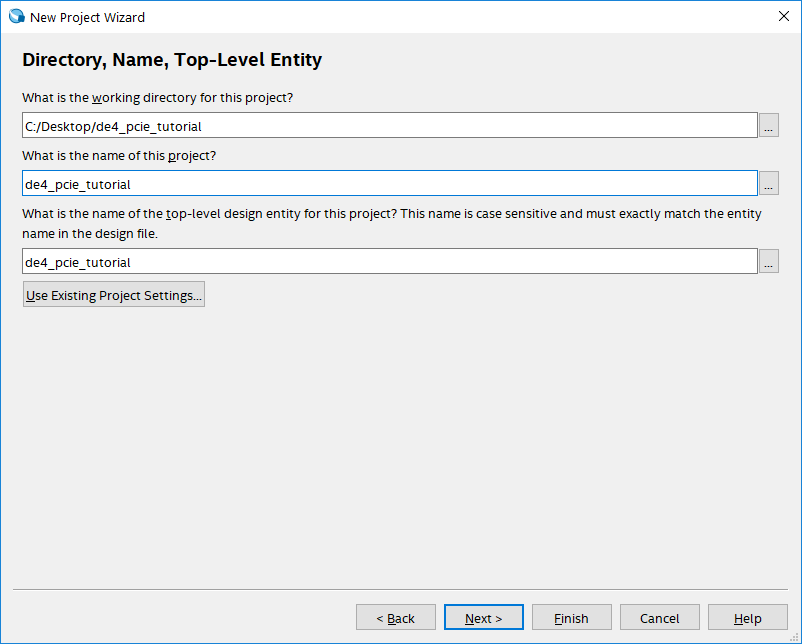
\includegraphics[scale=0.65]{figures/create_project.png}
	\caption{Create a new project.} 
	\label{fig:create_project}
\end{figure}

\begin{table}[H]
	\centering
	\caption{DE4 FPGA device names}
	\begin{tabular}{| c | c |}
		\hline
		Board & Device Name \\
		\hline
		DE4-230 & Stratix\textsuperscript{\textregistered} IV GX EP4SGX230KF40C2 \\
		\hline
		DE4-530 & Stratix\textsuperscript{\textregistered} IV GX EP4SGX530KH40C2 \\
		\hline
	\end{tabular}
	\label{tab:device}
\end{table}

\subsection{Creating a Platform Designer System}
In this section, we build a system with the PCI Express IP Core, DMA Controller, Scatter-Gather DMA Controller, on-chip memory, and the Nios II processor in Platform Designer. Select {\bf Tools} > {\bf Platform Designer} to open the Platform Designer as shown in Figure~\ref{fig:open_qsys}, and then save the file as {\it qsys\_system.qsys}. 

\begin{figure}[H]
	\centering
	  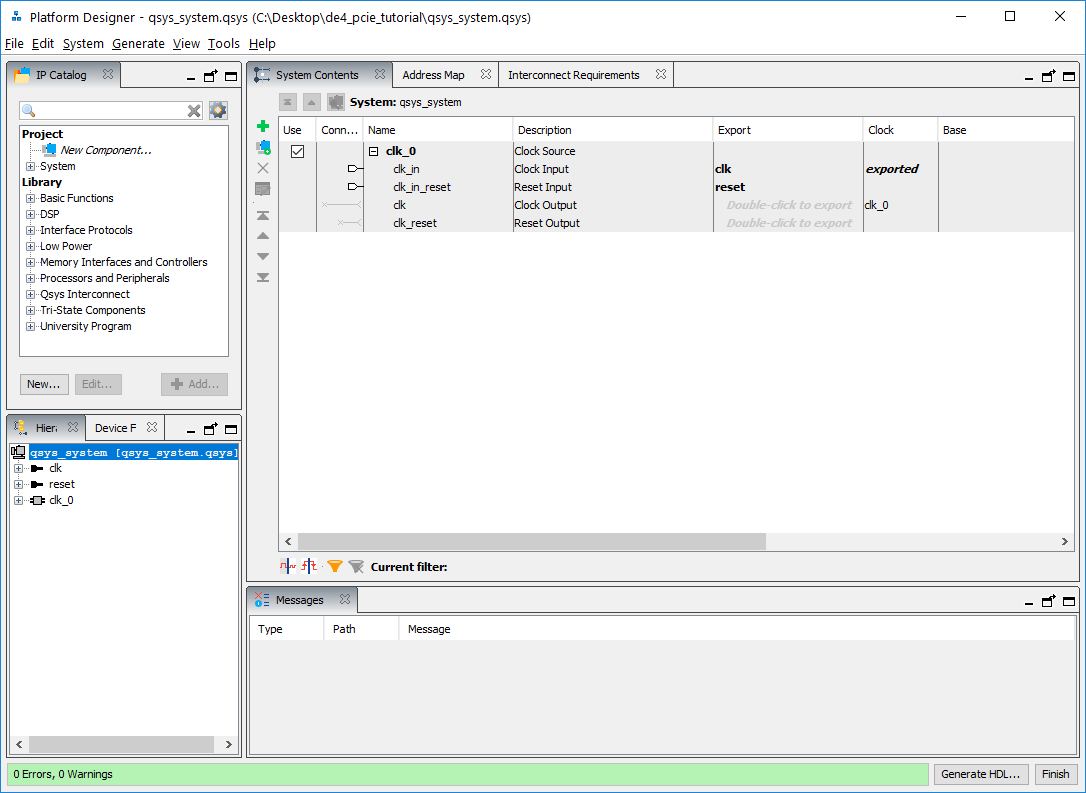
\includegraphics[scale=0.60]{figures/open_qsys.png}
	\caption{Open the Platform Designer tool.} 
	\label{fig:open_qsys}
\end{figure}

To add the PCI Express IP Core, perform the following:

\begin{itemize}
	\item Select {\bf Interface Protocols} > {\bf PCI Express} > {\bf IP Compiler for PCI Express} and click {\bf Add}. The Configuration Wizard window appears. You can use the scroll bar on the right to view parameters that are not initially visible.
	\item Under the {\bf System Settings} heading, set the {\bf Test out width} to {\it None} and leave others as default. 
	\item Under the {\bf PCI Base Address Registers} heading, set {\bf BAR0} as {\it 64 bit Prefetchable Memory} and {\bf BAR2} as {\it 32 bit Non-Prefetchable}. 
	\item Under the {\bf Device Identification Registers} heading, set the {\bf Device ID} to {\it 0x00000de4}.
	\item Under the {\bf Address Translation} heading, set the {\bf Address translation table configuration} to {\it Dynamic translation table}, {\bf Number of address pages} to {\it 2} and the {\bf Size of address pages} to {\it 1 GByte - 30 bits}.
	\item Click {\bf Finish} to add the PCI Express IP Core {\it pcie\_hard\_ip\_0} to the Platform Designer system. Figure~\ref{fig:pcie_ip_settings} shows screenshots of the settings. 
\end{itemize}

\begin{figure}[H]
	\centering
	  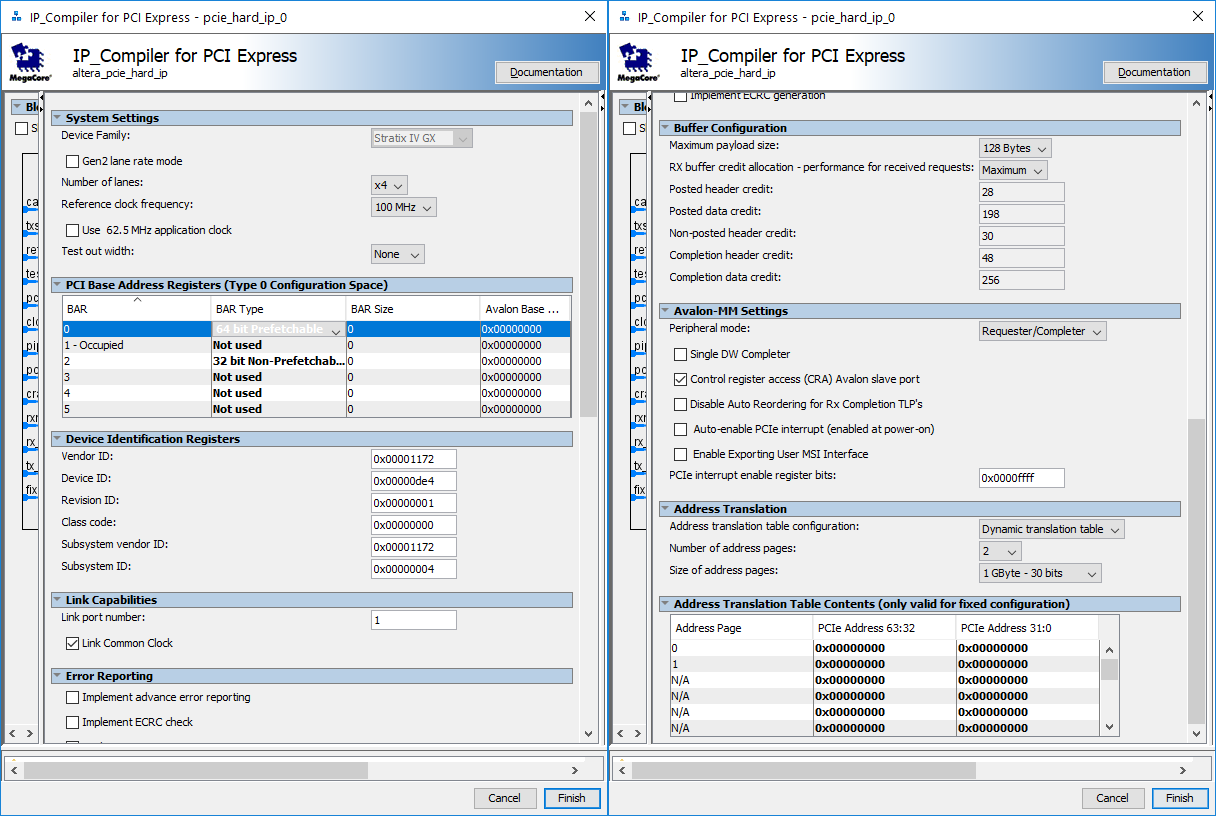
\includegraphics[scale=0.55]{figures/pcie_ip_settings.png}
	\caption{Settings for PCI Express IP Core.} 
	\label{fig:pcie_ip_settings}
\end{figure}

To add the DMA Controller, perform the following:
	
\begin{itemize}
	\item Select {\bf Basic Functions} > {\bf DMA} > {\bf DMA Controller Intel FPGA IP} and click {\bf Add}. 
	\item Under the {\bf DMA Parameters} tab, check the checkbox {\bf Enable burst transfers} and set the {\bf Maximum burst size} to 1024 words. 
	\item Select the {\bf Advanced} tab, and uncheck all the checkboxes except {\bf doubleword}. This makes the DMA Controller allow for doubleword (64 bits) transactions only.
	\item Click {\bf Finish}, then the DMA Controller {\it dma\_0} is added to the Platform Designer system. Figure~\ref{fig:dma_settings} shows the screenshots of the settings. 
\end{itemize}

\begin{figure}[H]
	\centering
	  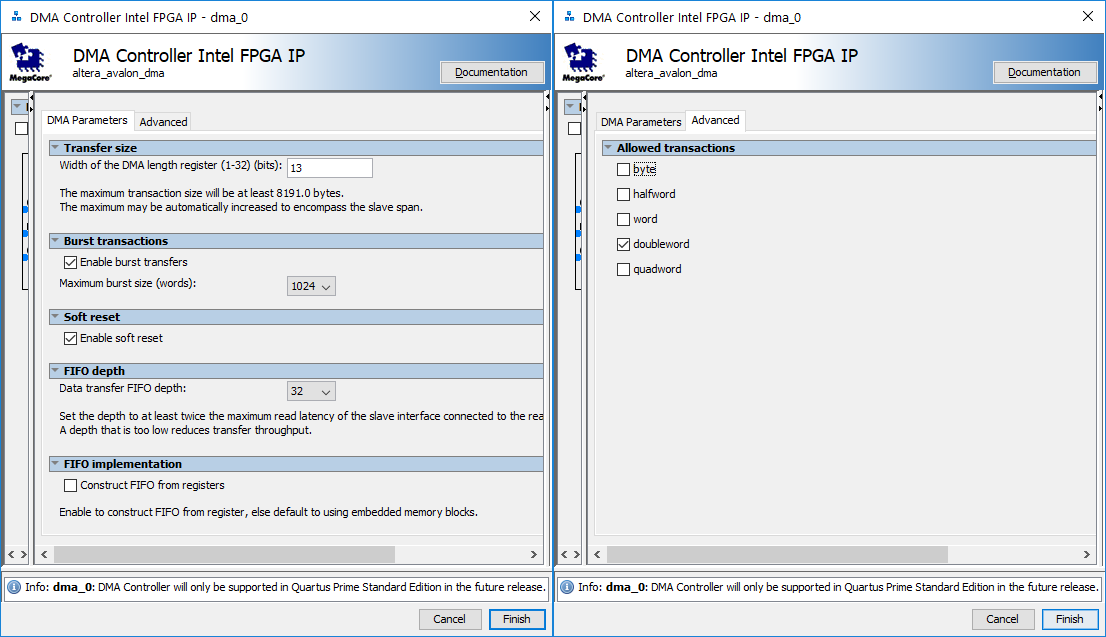
\includegraphics[scale=0.6]{figures/dma_settings.png}
	\caption{Settings for DMA Controller.} 
	\label{fig:dma_settings}
\end{figure}
	
To add the Scatter-Gather DMA Controller, perform the following: 

\begin{itemize}
	\item Select {\bf Basic Functions} > {\bf DMA} > {\bf Scatter-Gather DMA Controller Intel FPGA IP} and click {\bf Add}.
	\item In the Configuration Wizard window, check the checkbox of {\bf Enable burst transfers} and set the {\bf Data width} to 32 as shown in Figure~\ref{fig:sgdma_settings}.
	\item Click {\bf Finish}, then the Scatter-Gather DMA Controller {\it sgdma\_0} is added to the Platform Designer system.
\end{itemize}

\begin{figure}[H]
	\centering
	  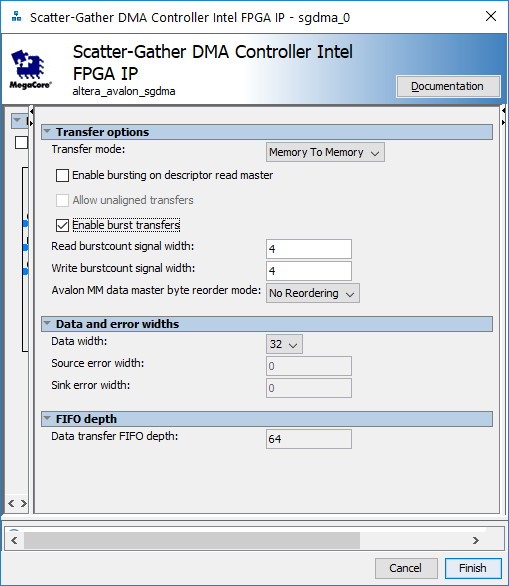
\includegraphics[scale=0.65]{figures/sgdma_settings.png}
	\caption{Settings for Scatter-Gather DMA Controller.} 
	\label{fig:sgdma_settings}
\end{figure}

To add the on-chip memory, perform the following:

\begin{itemize}
	\item Select {\bf Basic Functions} > {\bf On Chip Memory} > {\bf On-chip Memory(RAM or ROM) Intel FPGA IP} and click {\bf Add}.
	\item In the Configuration Wizard window, check the checkbox of {\bf Dual-port access}. This will enable the on-chip memory to support two different clock signals. 
	\item Set the {\bf Slafe S1 Data width} to {\it 64 bits} and the {\bf Total Memory Size} to {\it 8 Kbytes (8192 bytes)}.
	\item Check the check box of {\bf Enable non-default initialization file} and set the {\bf User created initialization file} to {\it onchip\_memory2\_0.hex} as shown in Figure~\ref{fig:onchip_mem_settings}.
	\item Click {\bf Finish}, then the on-chip memory {\it onchip\_memory2\_0} is added to the Platform Designer system.
\end{itemize}

\begin{figure}[H]
	\centering
	  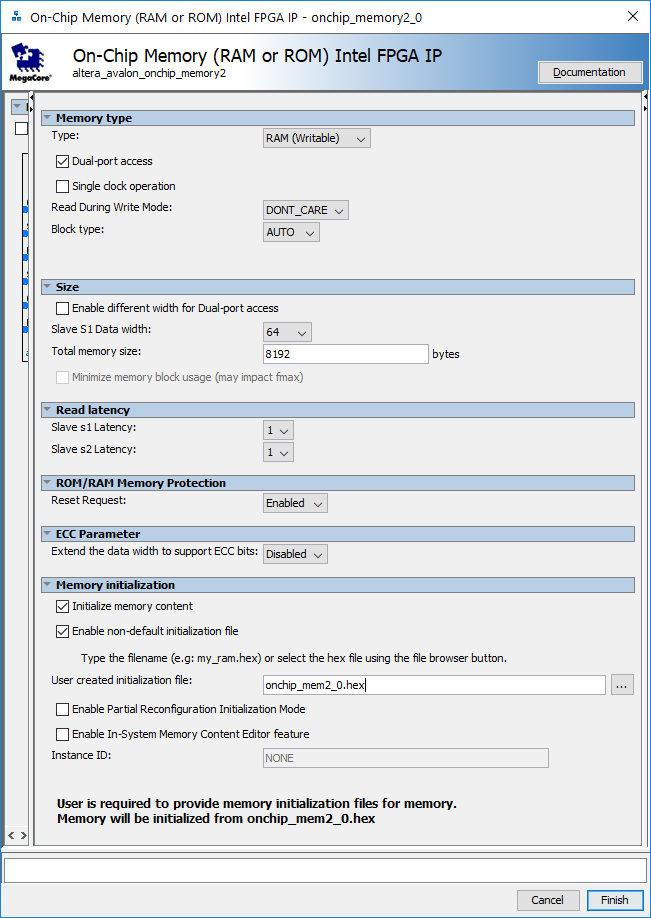
\includegraphics[scale=0.55]{figures/onchip_mem_settings.png}
	\caption{Settings for On-chip Memory.} 
	\label{fig:onchip_mem_settings}
\end{figure}

To add the Nios II processor, perform the following:

\begin{itemize}
	\item Select {\bf Processors and Peripherals} > {\bf Embedded Processors} > {\bf Nios II Processor} and click {\bf Add}.
	\item Choose {\bf Nios II/e}, which is the simplest version of the processor.
	\item Click {\bf Finish} to add the Nios II Processor {\it nios2\_qsys\_0} to the Platform Designer system. There may be some error messages at the bottom of the screen, because some parameters have not been specified yet. Ignore these messages as we will provide the necessary data later. 
\end{itemize}

\newpage
Note that the Platform Designer automatically chooses names for the components. The name are not necessarily descriptive enough for the design, but they can be changed. To rename a component, right-click the component name and select {\bf Rename}. Change the names of your components to the names shown in Figure~\ref{fig:qsys_system_renamed}.

\begin{figure}[H]
	\centering
	  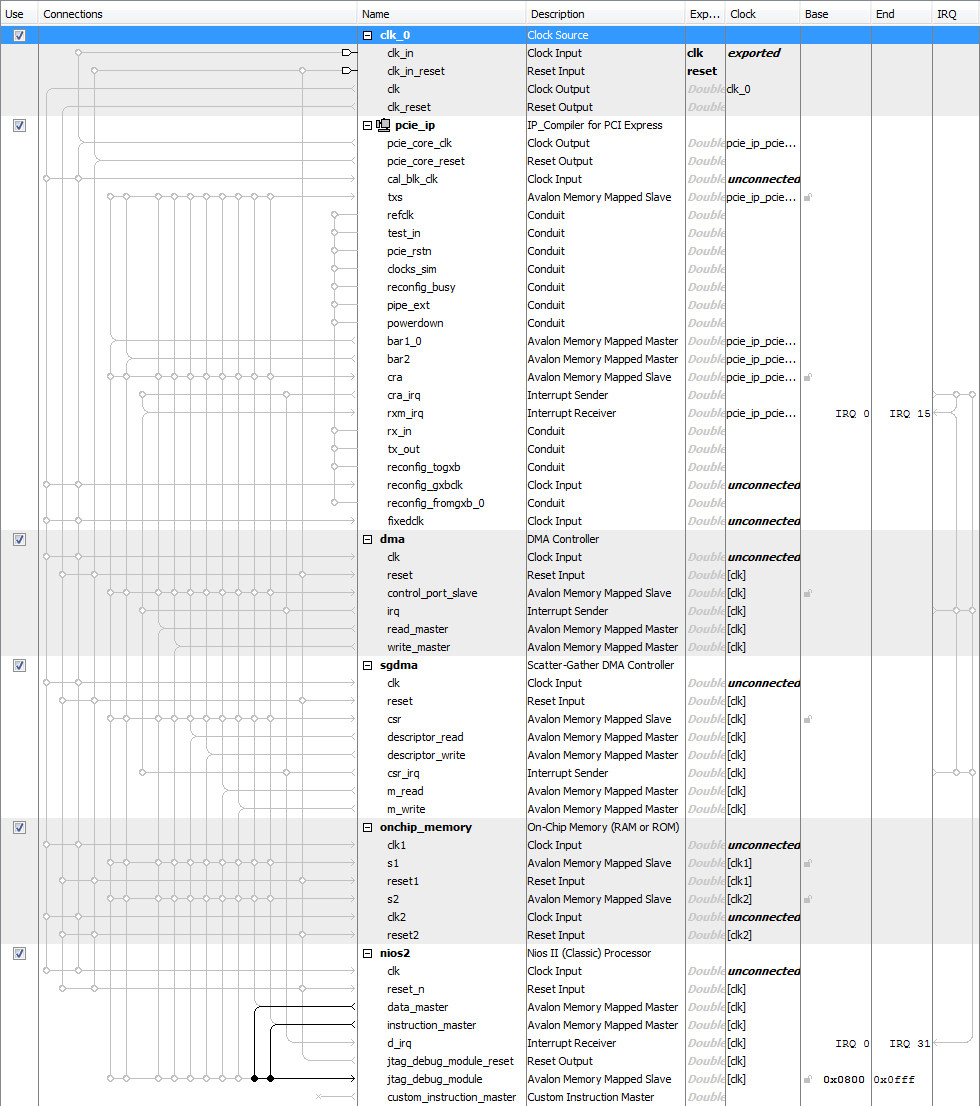
\includegraphics[scale=0.53]{figures/qsys_system_renamed.png}
	\caption{The Platform Designer system with renamed components.} 
	\label{fig:qsys_system_renamed}
\end{figure}

After adding components, you have to connected them correctly. In Platform Designer, the {\bf Connections} column displays the potential connection points between components. A filled dot shows that a connection is made, while an open dot shows a potential connection point. To complete the connections in the Platform Designer system, follow these steps:

\begin{enumerate}
	\item Connect the {\bf pcie\_ip} {\it bar1\_0} Avalon\textsuperscript{\textregistered} MM master port to the {\bf onchip\_memory} {\it s1} Avalon MM slave port using the following procedures:
	
\begin{enumerate}
	\item Right-click the {\bf IP Compiler for PCI Express} component {\bf pcie\_ip}, hover in the {\bf Connections} and then the {\bf pcie\_ip.bar1\_0} to display possible connections. 
	\item Select the {\bf onchip\_memory.s1} on the list appeared.
\end{enumerate}

	\item Repeat step 1 to make the remaining connections listed in Table~\ref{tab:qsys_connections}.
	
\begin{table}[H]
	\centering
	\caption{Complete list of Platform Designer connections}
	\begin{tabular}{| l | l |}
		\hline
		{\bf Make Connection From:} & {\bf To:} \\
		\hline
		{\it clk\_50.clk} & {\it pcie\_ip.cal\_blk\_clk} \\
		\hline
		{\it clk\_50.clk}  & {\it onchip\_memory.clk2}\\
		\hline
		{\it clk\_50.clk} & {\it nios2.clk} \\
		\hline
		{\it clk\_50.clk\_reset} & {\it onchip\_memory.reset2}\\
		\hline
		{\it clk\_50.clk\_reset} & {\it nios2.reset\_n} \\
		\hline
		{\it pcie\_ip.pcie\_core\_clk}  & {\it onchip\_memory.clk1}  \\
		\hline
		{\it pcie\_ip.pcie\_core\_clk}  & {\it dma.clk}  \\
		\hline
		{\it pcie\_ip.pcie\_core\_clk}  & {\it sgdma.clk}  \\
		\hline
		{\it pcie\_ip.pcie\_core\_reset} & {\it onchip\_memory.reset1} \\
		\hline
		{\it pcie\_ip.pcie\_core\_reset} & {\it dma .reset}  \\
		\hline
		{\it pcie\_ip.pcie\_core\_reset} & {\it sgdma.reset}  \\
		\hline
		{\it pcie\_ip.bar1\_0} (step 2) & {\it onchip\_memory.s1}  \\
		\hline
		{\it pcie\_ip.bar2}& {\it dma.control\_port\_slave} \\
		\hline
		{\it pcie\_ip.bar2}  & {\it pcie\_ip.cra} \\
		\hline
		{\it pcie\_ip.bar2}  & {\it sgdma.csr}  \\		
		\hline
		{\it dma.read\_master}  & {\it onchip\_memory.s1} \\
		\hline
		{\it dma.read\_master}  & {\it pcie\_ip.txs}  \\
		\hline
		{\it dma.write\_master}  & {\it onchip\_memory.s1}  \\
		\hline
		{\it dma.write\_master} & {\it pcie\_ip.txs}  \\
		\hline
		{\it sgdma.descriptor\_read}  & {\it pcie\_ip.txs} \\
		\hline
		{\it sgdma.descriptor\_write}  & {\it pcie\_ip.txs}  \\
		\hline
		{\it sgdma.m\_read} & {\it onchip\_memory.s1}\\
		\hline
		{\it sgdma.m\_read}  & {\it pcie\_ip.txs}  \\
		\hline
		{\it sgdma.m\_write}  & {\it onchip\_memory.s1}\\
		\hline
		{\it sgdma.m\_write} & {\it pcie\_ip.txs}  \\
		\hline
		{\it nios2.data\_master} & {\it onchip\_memory.s2} \\
		\hline
		{\it nios2.instruction\_master} & {\it onchip\_memory.s2} \\
		\hline
	\end{tabular}
	\label{tab:qsys_connections}
\end{table}
	
	\item In the {\bf IRQ} panel, click the connection from the Interrupt Sender of the {\it dma} component to the Interrupt Receiver {\it pcie\_ip} component and type 1 into the box. Because the Platform Designer-generated IP Compiler for PCI Express implements an individual interrupt scheme, you must specify the bit to which interrupt connects. In this case, the DMA Controller's interrupt sender signal connects to bit 1 of the IP Compiler for PCI Express input interrupt bus. 
	\item In the {\bf IRQ} panel, connect the Interrupt Sender of the {\it sgdma} component to the Interrupt Receiver {\it pcie\_ip} component and type 2. 
	
\end{enumerate}

Besides connections inside the Platform Designer system, there are signals that have to be exported to make connections outside the system. To export signals, follow the steps: 

\begin{enumerate}
	\item In the row of the signal you want to export, click the {\bf Export} column.
	\item Accept the default name that appears in the {\bf Export} column by clicking outside the cell without modifying the text.
\end{enumerate}

Export the {\it pcie\_ip} interfaces listed in Table~\ref{tab:qsys_exported}. After the signals are connected or exported, your Platform Designer system should appear as indicated in Figure~\ref{fig:qsys_system_connected}.

\begin{table}[H]
	\centering
	\caption{List of the exported interfaces}
	\begin{tabular}{| l | l |}
		\hline
		{\bf Interface Name} & {\bf Exported Name} \\
		\hline
		{\it refclk} & {\it pcie\_ip\_refclk} \\
		\hline
		{\it test\_in} & {\it pcie\_ip\_test\_in} \\
		\hline
		{\it pcie\_rstn} & {\it pcie\_ip\_pcie\_rstn} \\
		\hline
		{\it clocks\_sim} & {\it pcie\_ip\_clocks\_sim} \\
		\hline
		{\it reconfig\_busy} & {\it pcie\_ip\_reconfig\_busy} \\
		\hline
		{\it pipe\_ext} & {\it pcie\_ip\_pipe\_ext} \\
		\hline
		{\it rx\_in} & {\it pcie\_ip\_rx\_in} \\
		\hline
		{\it tx\_out} & {\it pcie\_ip\_tx\_out} \\
		\hline
		{\it reconfig\_togxb} & {\it pcie\_ip\_reconfig\_togxb} \\
		\hline
		{\it reconfig\_gxbclk} & {\it pcie\_ip\_reconfig\_gxbclk} \\
		\hline
		{\it reconfig\_fromgxb\_0} & {\it pcie\_ip\_reconfig\_fromgxb\_0} \\
		\hline
		{\it fixedclk} & {\it pcie\_ip\_fixedclk} \\
		\hline
	\end{tabular}
	\label{tab:qsys_exported}
\end{table}

\begin{figure}[H]
	\centering
	  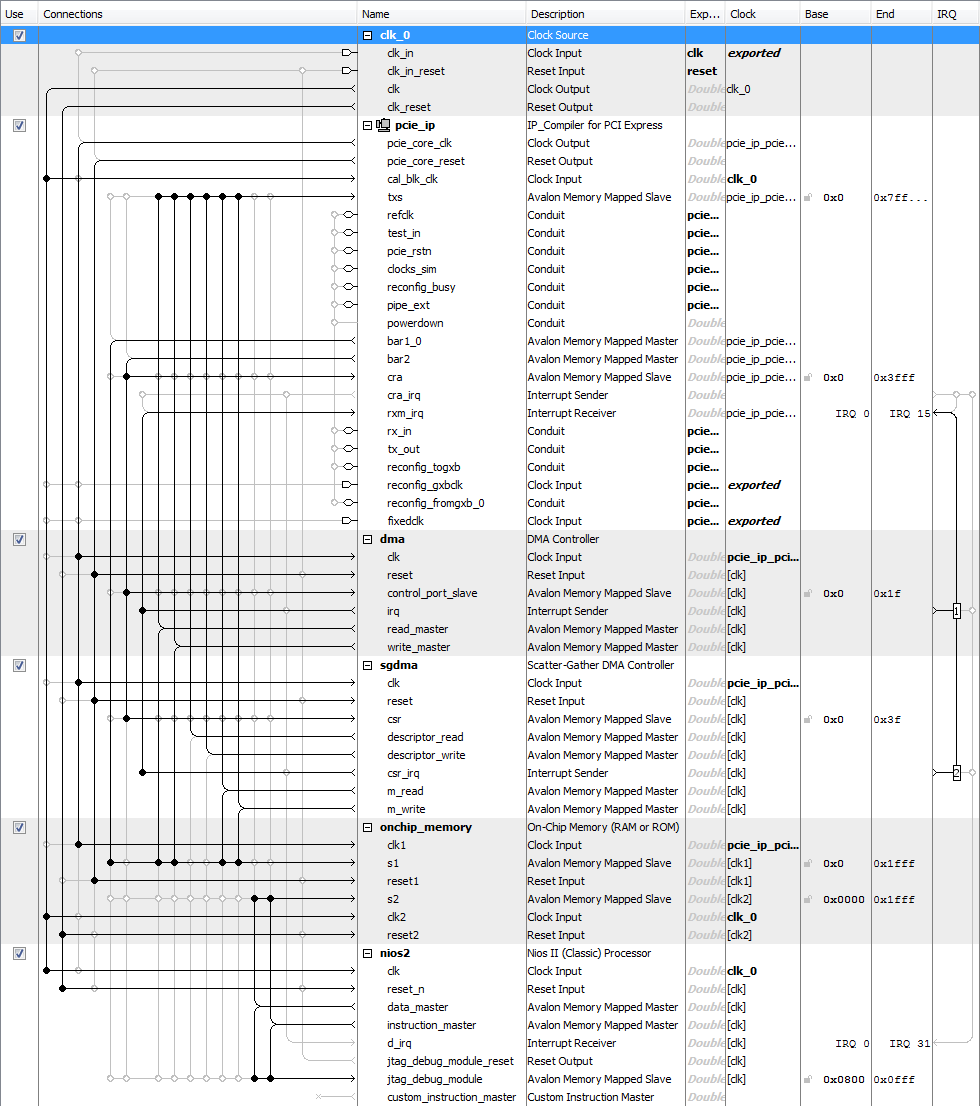
\includegraphics[scale=0.6]{figures/qsys_system_connected.png}
	\caption{The Platform Designer system with connections.} 
	\label{fig:qsys_system_connected}
\end{figure}

Before you can generate the Platform Designer system, You notice that there are still some errors in the message box. Platform Designer requires that you resolve the base addresses of all Avalon MM slave interfaces in the Platform Designer system. You can either use the auto-assign feature, or specify the base addresses manually. To use the auto-assign feature, on the {\bf System} menu, click {\bf Assign Base Addresses}. Figure~\ref{fig:qsys_address_map} shows the desired {\bf Address Map} tab of the Platform Designer system after you have auto-assigned the base address. Make any changes needed to ensure that all addresses match those in Figure~\ref{fig:qsys_address_map} before continuing.

\begin{figure}[H]
	\centering
	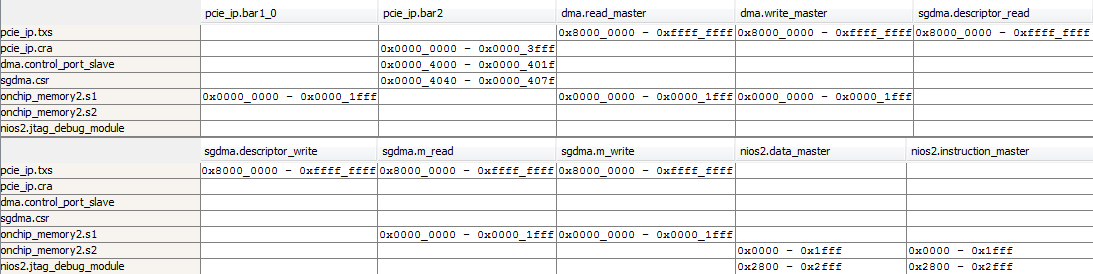
\includegraphics[scale=0.55]{figures/qsys_address_map.png}
	\caption{The Platform Designer Address Map.} 
	\label{fig:qsys_address_map}
\end{figure}

Also, you have to define the behaviour of the Nios II processor. Double-click on the {\it nios2} component and then select {\bf onchip\_memory.s2} to be the memory device for both reset vector and exception vector, as shown in Figure~\ref{fig:nios2_settings}. The reset vector is the location in the memory device the processor fetches the next instruction when it is reset. Similarly, the exception vector is the memory address the processor goes to when an interrupt is raised.

\begin{figure}[H]
	\centering
	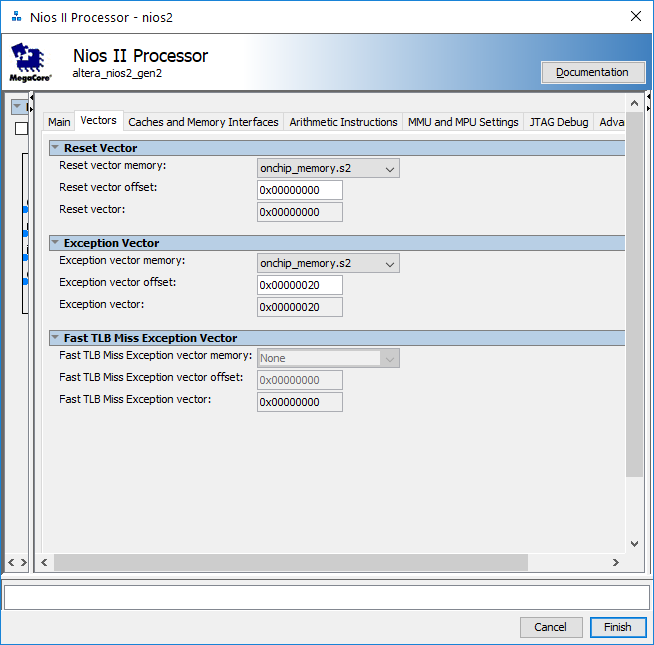
\includegraphics[scale=0.55]{figures/nios2_settings.png}
	\caption{The Settings for Nios II processor.} 
	\label{fig:nios2_settings}
\end{figure}

Now, the error messages should disappear and your Platform Designer system is finished. To generate the system, perform the following:

\begin{enumerate}
	\item Select {\bf Generate > Generate HDL}, uncheck the {\bf Create block symbol file (.bsf)} in the {\bf Synthesis} section as shown in Figure~\ref{fig:qsys_system_generation}.
	\item Click the {\bf Generate} button at the bottom of the tab.
	\item After Platform Designer reports {\bf Generate Completed} in the {\bf Generate} progress box title, click {\bf Close}.
	\item On the {\bf File} menu, click {\bf Save} and then close the Platform Designer application.
\end{enumerate}

\begin{figure}[H]
	\centering
	  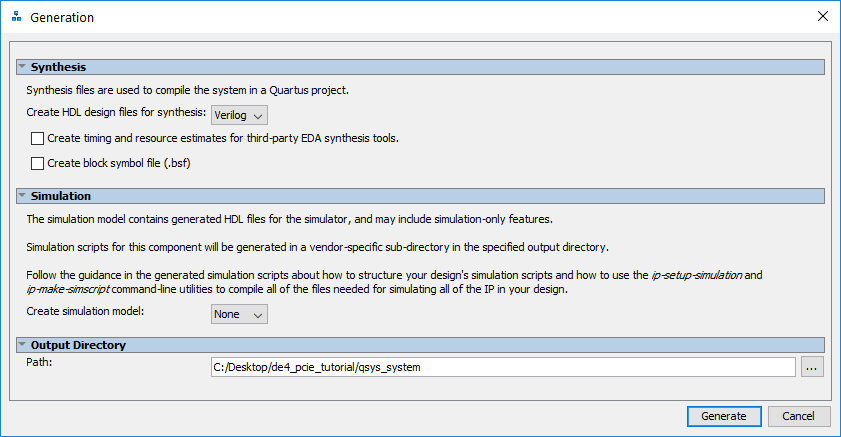
\includegraphics[scale=0.65]{figures/qsys_system_generation.png}
	\caption{The Platform Designer Generation tab.} 
	\label{fig:qsys_system_generation}
\end{figure}

\subsection{Adding PLL Using IP Catalog}
Besides the Platform Designer system, you need to add a Phase-locked loop (PLL) block, which is not added as a Platform Designer component. The PLL block is used to provide different clock signals for the Platform Designer system. To add the PLL block, perform the following:

\begin{enumerate}
	\item Select {\bf Tools} > {\bf IP Catalog}. %Select {\bf Create a new custom megafunction variation} when the window appears, and then click {\bf Next}.
	%\item Expand the {\bf I/O} directory under {\bf Installed Plug-Ins} by clicking the + icon left of the directory name, and click {\bf ALTPLL}.
	\item In the pop-up panel, select {\bf Library > Basic Functions > Clocks; PLLs and Resets > PLL > ALTPLL} and click {\bf Add...} button.
	\item Choose the {\bf Verilog} as the output file type for your design, and specify a variation name for output files. For this walkthrough, specify {\it my\_pll.v} as the name of the IP core file: <working\_dir>/my\_pll.v, as shown in Figure~\ref{fig:megawizard_pll}, and click {\bf OK}.

\begin{figure}[H]
	\centering
	  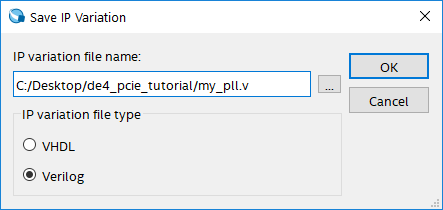
\includegraphics[scale=0.65]{figures/megawizard_pll.png}
	\caption{The IP Core Plug In Manager.} 
	\label{fig:megawizard_pll}
\end{figure}

	\item Under the {\bf Parameter Settings} tab, set {\bf What is the frequency of the inclk0 input} to 50MHz as shown in Figure~\ref{fig:mega_pll_settings_1} and click {\bf Next} to go to the {\bf Inputs/Lock} section.
	
\begin{figure}[H]
	\centering
	  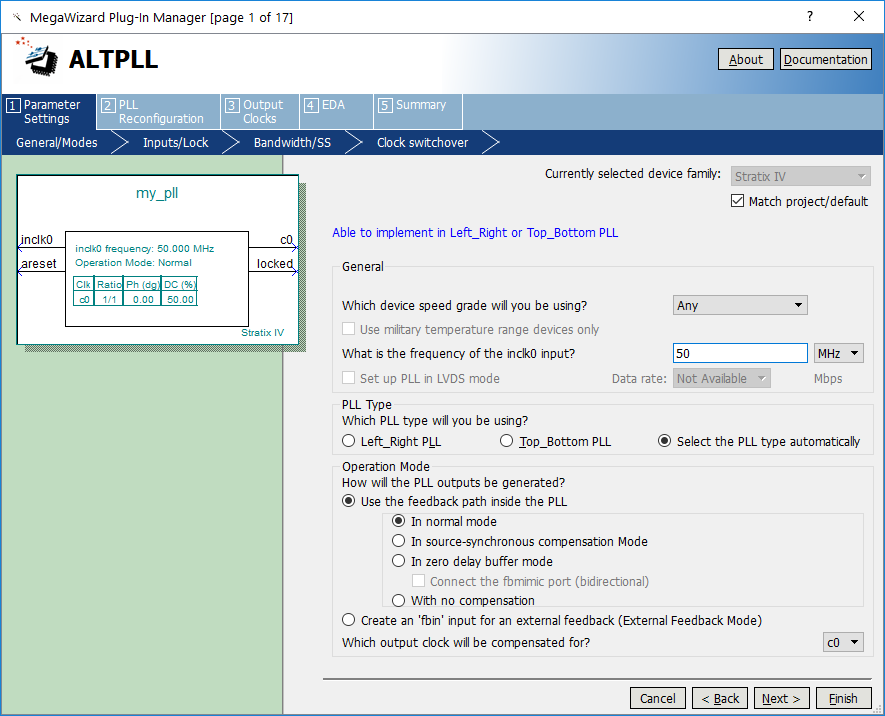
\includegraphics[scale=0.65]{figures/mega_pll_settings_1.png}
	\caption{Settings for General/Mode section.} 
	\label{fig:mega_pll_settings_1}
\end{figure}

	\item Uncheck the checkboxes of {\bf Create an `areset' input to asynchronously reset the PLL} and {\bf Create `locked' output} as shown in Figure~\ref{fig:mega_pll_settings_2}.
	
\begin{figure}[H]
	\centering
	  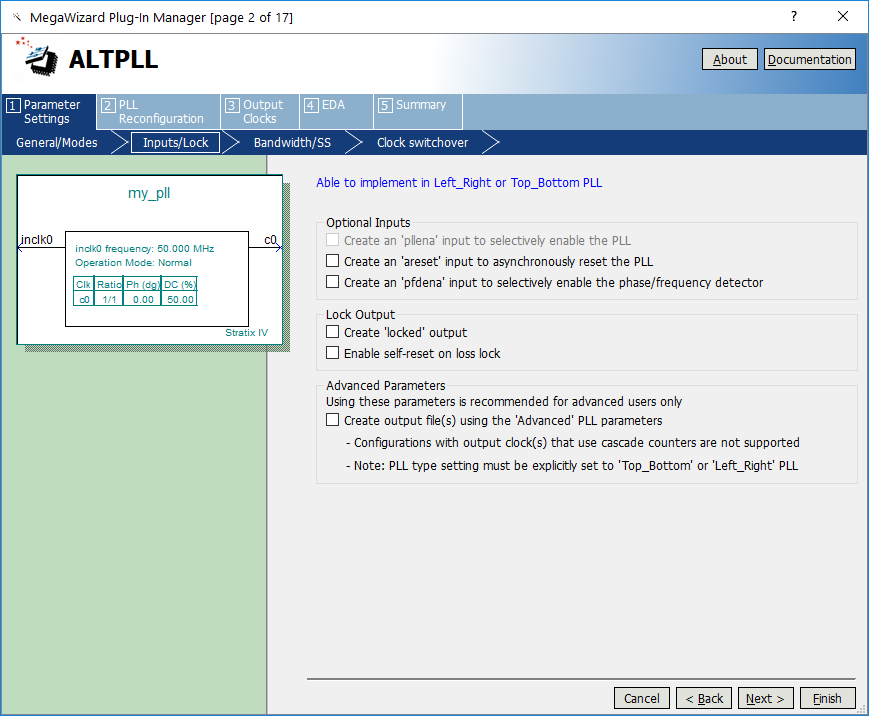
\includegraphics[scale=0.65]{figures/mega_pll_settings_2.png}
	\caption{Settings for Input/Lock section.} 
	\label{fig:mega_pll_settings_2}
\end{figure}
	
	\item Under the {\bf Output Clocks} tab, enter 50MHz after selecting {\bf Enter output clock frequency} as shown in Figure~\ref{fig:mega_pll_settings_3}, and click {\bf Next} to go to the {\bf clk\_c1} section.

\begin{figure}[H]
	\centering
	  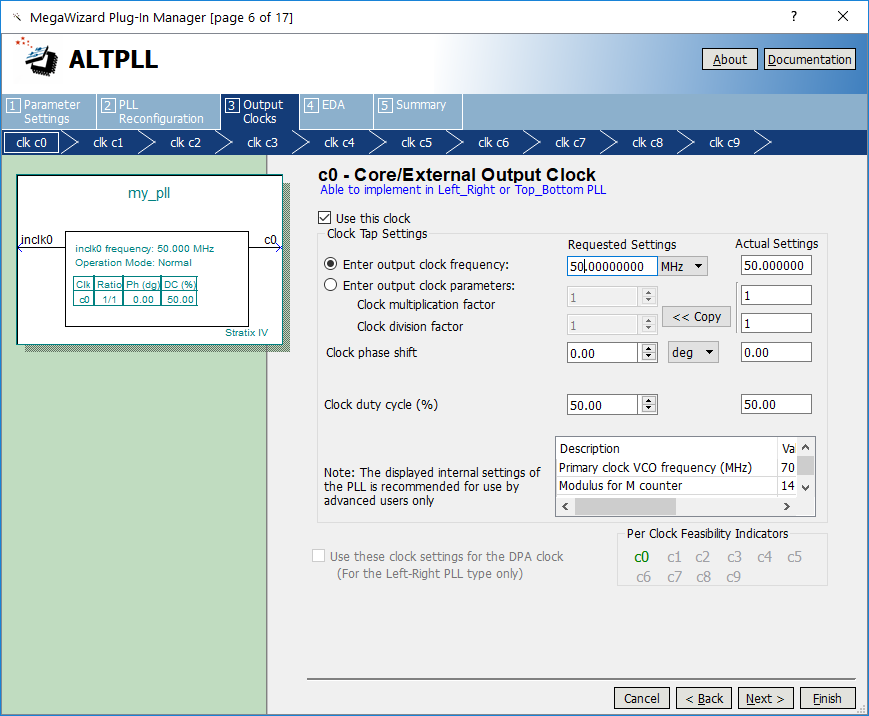
\includegraphics[scale=0.65]{figures/mega_pll_settings_3.png}
	\caption{Settings for output c0.} 
	\label{fig:mega_pll_settings_3}
\end{figure}

	\item Select the checkbox of {\bf Use this clock} and then set the output clock frequency to 125MHz with the same procedures of the last step, and click {\bf Next} to go to the {\bf clk\_c2} section.
	\item Select the checkbox of {\bf Use this clock} and then set the output clock frequency to 100MHz with the same procedures of the last step.
	\item Under the {\bf Summary} tab, uncheck {\bf my\_pll\_bb.v} as shown in Figure~\ref{fig:mega_pll_settings_4}, and then click {\bf Finish} to generate the file.
	
\begin{figure}[H]
	\centering
	  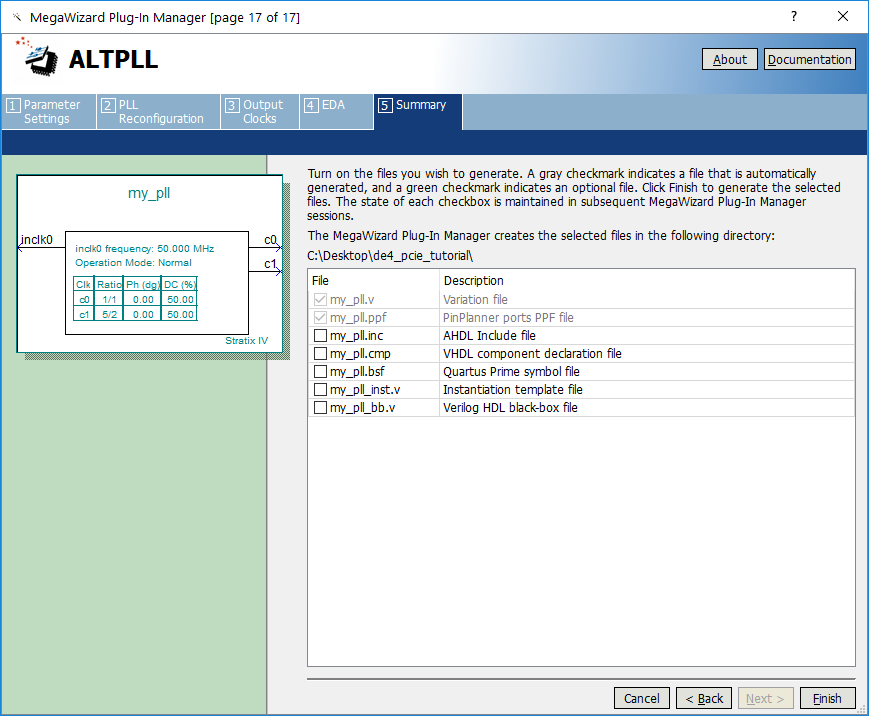
\includegraphics[scale=0.65]{figures/mega_pll_settings_4.png}
	\caption{Settings for Summary tab.} 
	\label{fig:mega_pll_settings_4}
\end{figure}

\end{enumerate}


\subsection{Integrating modules into the Quartus\textsuperscript{\textregistered} Prime Project}
To complete your hardware design, perform the following:

\begin{enumerate}
	\item Type the code in Figure~\ref{fig:wrapper_hdl} into a file called {\it de4\_pcie\_tutorial.v}. This code is a top-level Verilog module that instantiates the Platform Designer system and the PLL block. The module is named {\it de4\_pcie\_tutorial}, because this is the name we specified in Figure~\ref{fig:create_project} for the top-level design entity in the Quartus Prime project. 
	
\begin{figure}[H]%
	\lstinputlisting[language=Verilog, xleftmargin=2cm]{design_files/de4_pcie_tutorial.v}
	\caption{Verilog code for the top-level module}%
	\label{fig:wrapper_hdl}%
\end{figure}	
	
	\item Add the {\it de4\_pcie\_tutorial.v} file, the {\it qsys\_system.qip} file, the {\it my\_pll.qip} file, and the {\it onchip\_memory2\_0.hex} file to your Quartus Prime project as shown in Figure~\ref{fig:file_settings}. The {\it onchip\_memory2\_0.hex} file is used to initialize the on-chip memory and can be found in the directory {\it design\_files}, which can be downloaded along with this tutorial from the Intel FPGA University Program website. It contains the executable file of the demo application for the Nios II processor, which will be used in the next section.

\begin{figure}%
	\centering
		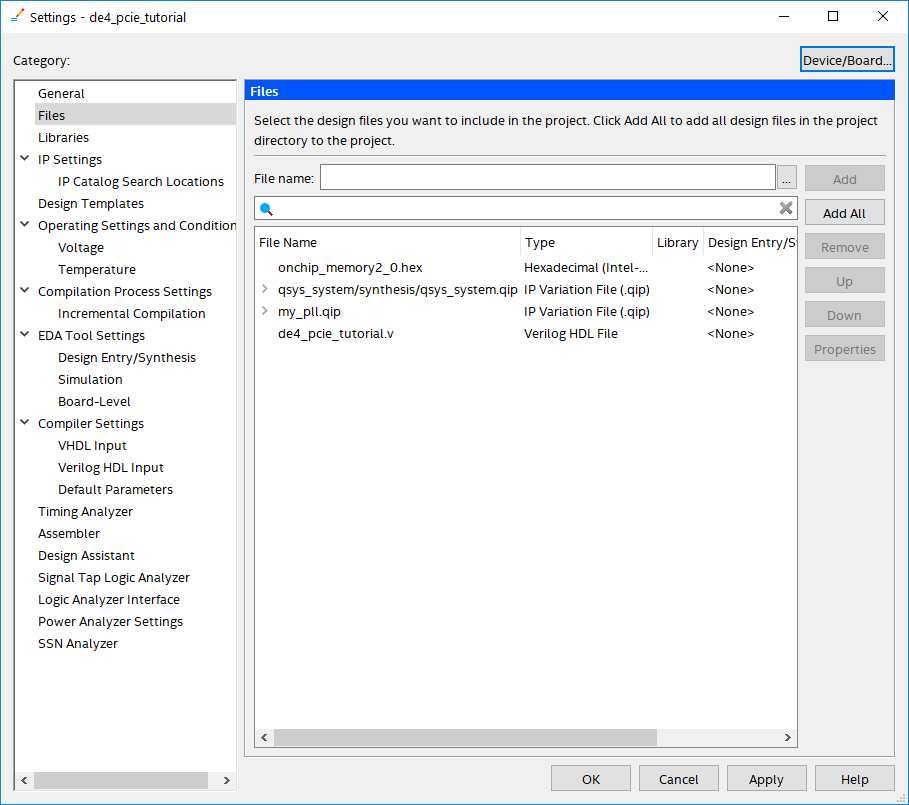
\includegraphics[scale=0.65]{figures/file_settings.png}%
	\caption{Files settings for the Quartus Project}%
	\label{fig:file_settings}%
\end{figure}

	\item Add the necessary pin assignments on the DE4 board to your project. Note that an easy way of making the pin assignments when you use the same pin names as in the DE4 User Manual is to import the assignments from file. The pin assignments can be found in the {\it DE4\_230\_pin\_assignments.qsf} or the {\it DE4\_530\_pin\_assignments.qsf} file (depending on your board), in the directory {\it design\_files}.
	\item Compile the Quartus Prime project.
\end{enumerate}

\subsection{Programming and Configuration}
\label{section:Programming and Configuration}
Before you can configure the DE4 board, you should plug the DE4 board into the PCI Express port of your Linux computer and connect the board to the computer by means of a USB cable plugged into the USB-Blaster port. Then turn on the power of the board and program the FPGA in the JTAG* programming mode as follows:
\begin{enumerate}
	\item Select {\bf Tools} > {\bf Programmer} to reach the window in Figure~\ref{fig:project_program}.
	
\begin{figure}%
	\centering
		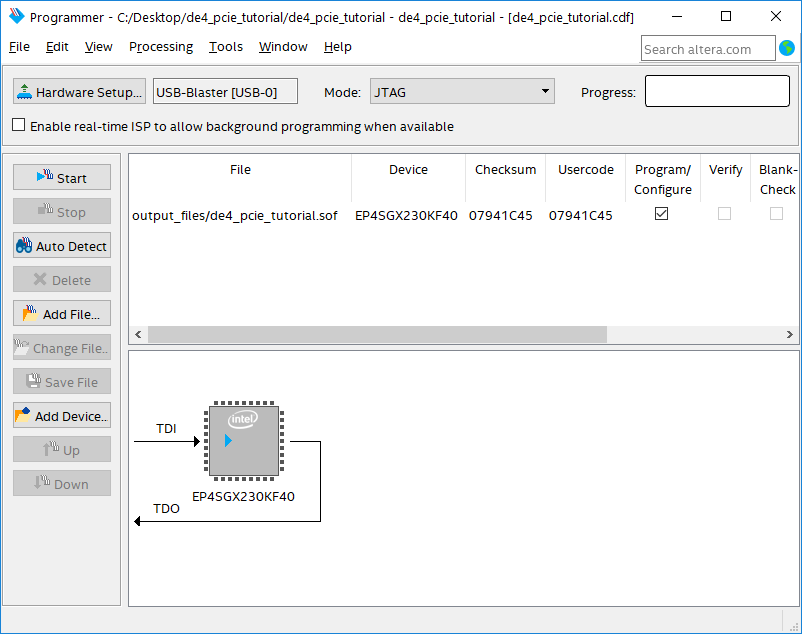
\includegraphics[scale=0.65]{figures/project_program.png}%
	\caption{The Programmer window.}%
	\label{fig:project_program}%
\end{figure}
	
	\item If the USB-Blaster is not chosen by default, press the {\bf Hardware Setup...} button and select the USB Blaster in the window that pops up.
	\item The configuration file {\it de4\_pcie\_tutorial.sof} should be listed in the window. If the file is not already listed, then click {\bf Add File} and select it from the {\it output\_files} subdirectory of the project. 
	\item At this point the window settings should appear as indicated in Figure~\ref{fig:project_program}. Press {\bf Start} to configure the FPGA.
	
\end{enumerate}

After you have successfully configured the hardware in the FPGA device, you should reboot your Linux computer to let the operating system to detect the PCI Express device you built. Ensure that the DE4 board is powered.

After the reboot, type command $lspci$ in the terminal to ask the operating system to list all the PCI devices on the computer. You should be able to see an Intel {\it 0xde4} device shown on the terminal.

\section{Using the Driver}
In the previous section, you have built a hardware system that supports the PCI Express; however, you need a driver to use the PCI Express to communicate with the DE4 board. Intel FPGA University Program provides an open source PCI driver for the usage of DE4 board in Linux operating system. The driver is designed to meet the general needs of using the PCI Express. It allows a user to:

\begin{enumerate}
	\item create a configuration file to define the hardware specific information for the driver.
	\item access any Base Address Registers (BAR). 
	\item use DMA Controller and Scatter-Gather DMA Controller.
	\item use either polling or interrupt for DMA transfers.
\end{enumerate}

The driver is in the directory {\it design\_files/driver}. The driver is tested on Linux 2.6.32, but it should work with newer versions of the Linux kernel. 

\subsection{Creating the Configuration File}
Before you can use the driver, you need to create a file to configure the driver for your hardware system. An example configuration file, {\it config\_file\_example}, can be found in the {\it driver} folder. To make the file for the system you built, open {\it config\_file\_example} and perform the following:

\begin{enumerate}
	\item Set the Vendor ID and Device ID. They should be the same with the IDs shown in Figure~\ref{fig:pcie_ip_settings}.   
		\begin{description}
			\item[vendor\_id = 0x1172]
			\item[device\_id = 0x0de4] 
		\end{description}
	\item Set the parameters related to the {\it PCI Express IP Core}.  
		\begin{description}
			\item[pci\_dma\_bit\_range = 31] This defines the bit mask for DMA buffers. By setting it to 31, you force Linux to allocate physical address between 0x00000000 $-$ 0x7FFFFFFF for DMA buffers. This parameter is decided by the settings of {\bf Address Translation} in the IP Compiler for PCI Express.  
			\item[tx\_base\_addr = 0x80000000] The base address of the {\it txs} Avalon MM slave.
			\item[pcie\_cra\_bar\_no = 2] This defines the number of the BAR which is connected to the {\it cra} Avalon MM slave.
			\item[pcie\_cra\_base\_addr = 0x00000000] The base address of {\it cra} Avalon MM slave.
		\end{description}
	\item Set the parameters for DMA controllers. By default, the driver supports at most four DMA controllers, so there are four columns in the {\it config\_file\_example}. You only need to fill in the first two columns for the {\it DMA Controller} and the {\it Scatter-Gather DMA Controller} in your system, and leave other columns as zeros. 
		\begin{description}
			\item[dma\_type = 1, 2] This defines the type of the DMA controller. The {\it DMA Controller} is represented by 1, while the {\it Scatter-Gather DMA Controller} is represented by 2.
			\item[dma\_irq\_no = 1, 2] This defines the interrupt number of DMA controller as shown Figure~\ref{fig:qsys_system_connected}. 
			\item[dma\_ctrl\_bar\_no = 2, 2] This defines the number of the BAR, which is connected to the control port of the DMA controller. 
			\item[dma\_ctrl\_base\_addr = 0x00004000, 0x00004040] This defines the base address of the control port.
		\end{description}
	\item Set the data width of the allowed transactions for {\it DMA Controller}. This is necessary if you are using the {\it DMA Controller}. 
		\begin{description}
			\item[sdma\_data\_width = 8, 0] Set the first number to 8 (words) to match the settings in Figure~\ref{fig:dma_settings} and ignore it for the {\it Scatter-Gather DMA Controller}. 
		\end{description}
	\item Save the file as tutorial\_config\_file.
\end{enumerate}

\subsection{Load the Driver Module into the Kernel}
To install the driver, you need to load the {\it .ko} module file into the Linux kernel. If it's your first time to use the driver, you have to compile the driver codes into the {\it .ko} module file. Run the makefile in the folder {\it driver} to compile the driver. Note that you may have to change the file format from the Windows* Format to the UNIX* Format first, so go to the demo and driver folders before compiling any programs, type:
	
$$ {\rm dos2unix~~*} $$

After you compiled the driver, you will get the kernel module file {\it alt\_up\_pci.ko}. The name of the module file is determined by the makefile and you are recommended not to change the name. Once you have the {\it .ko} module file, you don't have to recompile the driver for your future usage of the driver.

Each time you use the driver, you will have to dynamically load the driver module with the correct configuration file. This is done by a shell script {\it load\_alt\_up\_pci\_driver.sh} provided in the {\it driver} folder. Load the driver module with the configuration file you created by typing:
$$ {\rm sudo~~./load\_alt\_up\_pci\_driver.sh~~tutorial\_config\_file} $$
Note that you need to pass the file name of the configuration file as the first argument to the shell script, otherwise the script will use {\it config\_file} as default. If you have changed the makefile when compiling the driver codes, you have to modify the variable {\it DRV\_MODULE} in the shell script to match the name of your {\it .ko} module file. 

This script requires that your account has the administrator right. After typing in the password, you will see {\it Matching Device Found} on success, or {\it Matching Device Not Found} when failed. If the module is successfully loaded, the script will automatically create a character special file {\it alt\_up\_pci0} in directory {\bf /dev/}. This file is important because it represents the DE4 device and you will need to access it when you want to use the driver.

Since the driver is loaded into the kernel, the information printed out by the driver will not show on the terminal window directly. Instead, they will be printed as driver messages. To see the driver messages, type command:
$$ {\rm dmesg} $$
The driver messages are important messages to check the status of the driver especially when you encounter problems. You should be able to see similar driver messages shown in Figure~\ref{fig:dmesg_result} after you have loaded the driver module successfully.

\begin{figure}[H]%
	\centering
		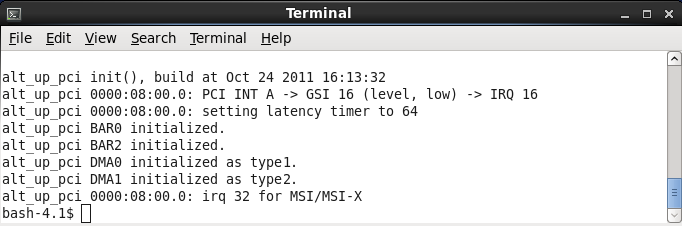
\includegraphics[scale=0.65]{figures/dmesg_result.png}%
	\caption{Messages shown on the terminal}%
	\label{fig:dmesg_result}%
\end{figure}

If you want to remove the module from the kernel, you can use the shell script below:
$$ {\rm sudo~~./unload\_alt\_up\_pci\_driver.sh} $$

\subsection{How to Use the Driver}
To help you understand how to use the driver, a demo application is provided. The application will ask you to input a sentence and the sentence will be sent to the on-chip memory of the DE4 board. Then the Nios II processor will change the sentence, modifying letters from lower-case to upper-case and vice versa. After the processing, the application will read the sentence back and print it on the screen. To ensure the data is shared correctly between the PC host and the DE4 board, one byte (0x00000FFF) in the on-chip memory is used to as a flag to indicate who owns the control of the data. `H' means the data is owned by the host while `B' means it's owned by the board. When the data is owned by one side, the other side should do nothing other than polling the control byte.

Figure~\ref{fig:demo_application} shows the simplified code of the demo application, which does not contain error checking. You can find the complete code {\it demo.c} in directory {\it design\_files/demo}.

\begin{figure}[H]
	\begin{lstlisting}[language=C, stepnumber=1, numbers=left]
#include <stdio.h>
#include <string.h>
#include "alt_up_pci_lib.h"

#define ONCHIP_CONTROL 0x00000FFF
#define ONCHIP_DATA 0x00001000
#define MAX_DATA_SIZE 4096
#define CTRLLER_ID 0

int main() {
    int fd, length_str;
    char buff[MAX_DATA_SIZE], control;

    alt_up_pci_open( &fd, "/dev/alt_up_pci0" );

    control = 'H'; // controlled by the host PC
    alt_up_pci_write( fd, BAR0, ONCHIP_CONTROL, &control, sizeof(control) );

    while(1) {
        fgets( buff, MAX_DATA_SIZE, stdin );
        length_buff = strlen(buff) + ( 8 0 - (strlen(buff)%8) );

        alt_up_pci_dma_add(fd, CTRLLER_ID, ONCHIP_DATA, buff, length_str, TO_DEVICE);
        alt_up_pci_dma_go (fd, CTRLLER_ID, INTERRUPT);

        control = 'B'; // pass the control right to the DE4 board
        alt_up_pci_write (fd, BAR0, ONCHIP_CONTROL, &control, sizeof(control) );

        while( control != 'H') // polling the control byte
            alt_up_pci_read( fd, BAR0, ONCHIP_CONTROL, &control, sizeof(control) );

        alt_up_pci_dma_add(fd, CTRLLER_ID, ONCHIP_DATA, buff, length_str, FROM_DEVICE);
        alt_up_pci_dma_go(fd, CTRLLER_ID, INTERRUPT) ;

        printf("Received : \n%s\n", buff);
    }

    alt_up_pci_close(fd);

    return 0;
}
	\end{lstlisting}
	\caption{Simplified code for demo application}%
	\label{fig:demo_application}%
\end{figure}

As you can see in Figure~\ref{fig:demo_application}, there are six functions prefixed with {\it alt\_up\_pci\_}. These functions are provided in the header file {\it alt\_up\_pci\_lib.h}. The descriptions of the functions are shown below. Note that all these functions will return $0$ on success, and return $-1$ when failed.

\begin{description}
	\item[alt\_up\_pci\_open()] -- This function is used to open the DE4 device file. 
	
	You will have to input the character special file of the device, which in this case is {\it alt\_up\_pci0}, then you will get a file descriptor. After calling this function successfully, you can start using other functions to perform operations on the DE4 board. 
	
	\item[alt\_up\_pci\_close()] -- This function used to close the DE4 device file.
	
	You will have to pass the file descriptor got from {\it alt\_up\_pci\_open()} to the function. This function should be called at the end of the application.  
	
	\item[alt\_up\_pci\_read()] -- This function is used to do the read operation. 
	
	You will have to select which BAR to read from and what is the starting address of the read operation. Also, you need to pass a pointer to the buffer and the size of the buffer to the function.
	
	\item[alt\_up\_pci\_write()] -- This function is used to do the write operation.
	
	This function is similar to {\it alt\_up\_pci\_read()} and does the write operation instead.
	
	\item[alt\_up\_pci\_dma\_add()] -- This function is used to add a DMA transfer into the queue of the DMA controller.
	
	Inside the driver, there is a queue for each DMA controller. You are allowed to push up to ten DMA transfers into the queue before the DMA controller really performs the transfers. You will need to pick a DMA controller to perform the transfer, and give it the pointer to the buffer, the address in the DE4 board, how many bytes you want to transfer and the direction of the transfer. Note that the driver will not check the overflow of the address, so the application is responsible to ensure that the DMA controller is not reading from or writing to an illegal address.	
	
	\item[alt\_up\_pci\_dma\_go()] -- This function is used to start the DMA transfers in the queue.
	
	By calling this function, the selected DMA controller will start performing all the DMA transfers in the queue, and it will use either polling or interrupt to check whether a transfer is finished. 
	
\end{description}

The header file {\it alt\_up\_pci\_lib.h} also contains three enum types for the BARs, the direction of the DMA, and the method of checking to increase the readability of the codes. We recommend you to include this file when you are writing your own application. 

Pay attention to the transfer length when using the {\it DMA Controller}, because the data length have to match the settings you made for the {\it DMA Controller}. In this tutorial, an error will occur, if the length is not a multiple of 8 or the address is not aligned with 8 bytes.

\subsection{Running the Demo Application}
To try the demo application, compile and run the demo codes in the {\it demo} folder. By typing sentence into the terminal and typing {\bf Enter} to send the sentence, you can see how the sentence is changed by the Nios II processor. You can also change the value of {\it CTRLLER\_ID} in the {\it demo.c} to select a different DMA controller.

The code shown in Figure~\ref{fig:demo_nios} is the code run by the Nios II processor. It is downloaded to the on-chip memory by adding the {\it onchip\_memory2\_0.hex} during the compile time. 

\begin{figure}[H]%
\begin{lstlisting}[language=C, stepnumber=1, numbers=left]
#include <stdio.h>

volatile char *onchip_control = (char *) 0x00000FFF;
volatile char *onchip_data = (char *) 0x00001000;

int main() {
    int i;
    char ch;

    while( 1 ) {
        while( *onchip_control != 'B' ) // polling the control byte
            ;

        i = 0;
        while( (ch = *(onchip_data + i) ) != '\n' ) {
            if ( ch >= 'a' && ch <= 'z' )
                *(onchip_data + i) = ch - 'a' + 'A';
            else if ( ch >= 'A' && ch <= 'Z' )
                *(onchip_data + i) = ch - 'A' + 'a';
            else
                *(onchip_data + i) = ch;
            i++;
        }

        *onchip_control = 'H' ; // pass the control right to the host PC
    }
    return 0;
}
\end{lstlisting}
	\caption{Program run by the Nios II Processor}%
	\label{fig:demo_nios}%
\end{figure}


\subsection{Reprogramming the FPGA without Rebooting the Host Computer}
After you successfully configure the FPGA and install the driver on your host computer, you may still want to modify your PCI Express settings on the FPGA and reprogram it. However, reprogramming the FPGA will disable the connection between the FPGA and the host computer. It requires you to reboot the host computer and reload the driver every time you download a new configuration onto the FPGA, which is inconvenient and time-consuming. Here we provide a way to reprogram the FPGA without rebooting the host computer if a valid PCI Express connection has already been established:
\begin{enumerate}
	\item To save the PCI Express registers, go to the demo folder, run: 
		$$ {\rm ./reprogram~~save} $$
	\item Program a new image(.sof) on FPGA following the instructions in section ~\ref{section:Programming and Configuration}.
	Note that the memory space, the Vendor ID and the Device ID of the PCI Express shouldn't be changed in Platform Designer, otherwise restoring the register information will give the wrong information to the host computer.
	\item Then we need to restore the registers information, go to the demo folder, run:
		$$ {\rm ./reprogram~~restore} $$
	\item Go to the driver folder to unload and reload the driver using:
		$$ {\rm ./unload\_alt\_up\_pci\_driver.sh} $$
		$$ {\rm ./load\_alt\_up\_pci\_driver.sh\ tutorial\_config\_file} $$
\end{enumerate}
The device connection should be re-established. 

\section{Changing the Driver}
Now, you can start building your own system and applications. However, if you are not satisfied with the functionality provided by the driver and want to design your custom driver, you can read the {\it index.html} in directory {\it design\_files/doc/html}. This file is generated by the Doxygen and it will give you a general idea of the driver, so that you can change it. 



% Copyright and Trademark

%\newcommand{\datePublished}{Mar 2022}

\newcommand{\versnum}{21.1} %version number quartus/AMP
\newcommand{\quartusname}{Quartus\textsuperscript{\textregistered} Prime}	
\newcommand{\textBar}{For \quartusname{} \versnum{}}
\newcommand{\thisyear}{2022 } %for copyright
\newcommand{\company}{FPGAcademy.org}
\newcommand{\longteamname}{FPGAcademy.org}
\newcommand{\teamname}{FPGAcademy}
\newcommand{\website}{FPGAcademy.org}

\newcommand{\productAcronym}{AMP}
\newcommand{\productNameShort}{Monitor Program}

\newcommand{\productNameMedTM}{Monitor Program}
\newcommand{\productNameMed}{Monitor Program}

%\newcommand{\headerLogoFilePath}[1]{#1/FPGAcademy.png}



%%%%%%%%%%%%%%%%%%%%%%%%%%%%%%%%%%%%%%%%
%%% FPGAcademy Copyright Information %%%
%%%%%%%%%%%%%%%%%%%%%%%%%%%%%%%%%%%%%%%%

%Always put the copyright on a new page (clear page), with some vertical space from top
\clearpage
\vspace{1in}

\noindent

Copyright {\copyright} FPGAcademy.org. All rights reserved. FPGAcademy and the FPGAcademy logo are trademarks of  FPGAcademy.org.  This document is being provided on an ``as-is'' basis and as an accommodation and therefore all warranties, representations or guarantees of any kind (whether express, implied or statutory) including, without limitation, warranties of merchantability, non-infringement, or fitness for a particular purpose, are specifically disclaimed.

%FPGAcademy assumes no responsibility or liability arising out of the application or use of any information,  product,  or  service  described  herein  except  as  expressly  agreed  to  in  writing  by  FPGAcademy.



**Other names and brands may be claimed as the property of others.




\end{document}
